\documentclass[aspectratio=169, UTF8, fontset=macnew, 11pt]{ctexbeamer}

\usetheme{Madrid}
\usecolortheme{seahorse}
\usefonttheme{professionalfonts}
\setbeamertemplate{navigation symbols}{}
\setbeamertemplate{caption}{\insertcaption}
\setbeamerfont{frametitle}{size=\large}
\setbeamerfont{title}{size=\Large}

\usepackage{amsmath, amssymb}
\usepackage{booktabs}
\usepackage{graphicx}
\usepackage{xcolor}

\graphicspath{{../output/figures/}}

\newcommand{\edag}{e_0^{\dagger}}
\newcommand{\LCe}{\text{LC}e^{\dagger}}
\newcommand{\hi}[1]{\textcolor{red!70!black}{\textbf{#1}}}
\newcommand{\gd}[1]{\textcolor{green!45!black}{\textbf{#1}}}

\title[小人口 LC 模型]{小人口 Lee-Carter 模型之估計與區間推論}
\subtitle{兼論修勻與壽命差異調整的適用界限}
\author[林子立]{林子立\\[4pt]\small 指導教授：余清祥\,教授}
\institute{國立政治大學統計學系}
\date{2026 年 9 月 21 日}

\begin{document}

\begin{frame}[plain]
\titlepage
\end{frame}

\begin{frame}{符號約定}
\begin{columns}[T]
\begin{column}{0.5\textwidth}
\small
索引：$x=1,\dots,A$（年齡組，$A=22$）、$t=1,\dots,T$（年份）。
\vspace{6pt}

\begin{itemize}\small
  \item \textbf{純量}細體小寫：$D_{x,t}$ 死亡數、$E_{x,t}$ 暴露數、
        $m_{x,t}=D_{x,t}/E_{x,t}$
  \item \textbf{向量}粗體小寫（行向量）：
        $\boldsymbol{\alpha},\boldsymbol{\beta}\in\mathbb{R}^{A}$、
        $\boldsymbol{\kappa}\in\mathbb{R}^{T}$
  \item \textbf{矩陣}粗體大寫：
        $\mathbf{D},\mathbf{E}\in\mathbb{R}^{A\times T}$
\end{itemize}
\vspace{4pt}
\footnotesize
\hi{附下標的 $\beta_x$、$\kappa_t$ 是向量的第 $x$（第 $t$）個分量}；
不附下標的粗體符號代表整個向量。$\mathbf{1}_A$ 為全一向量。
\end{column}
\begin{column}{0.48\textwidth}
\small
\textbf{Lee-Carter 模型}
\[
\log m_{x,t}=\alpha_x+\beta_x\kappa_t+\varepsilon_{x,t}
\]
以向量寫成
$\log\mathbf{M}=\boldsymbol{\alpha}\mathbf{1}_T^{\!\top}
+\boldsymbol{\beta}\boldsymbol{\kappa}^{\!\top}+\boldsymbol{\varepsilon}$
$\Rightarrow$ \gd{模型的秩為一}。
\vspace{8pt}

\textbf{識別條件}
\[
\mathbf{1}_A^{\!\top}\boldsymbol{\beta}=1,\qquad
\mathbf{1}_T^{\!\top}\boldsymbol{\kappa}=0
\]
\vspace{-6pt}
\begin{alertblock}{}
\footnotesize
第一式在懲罰式估計中\hi{扮演決定性的角色}——它使「朝零收縮」的懲罰項
退化為常數。
\end{alertblock}
\end{column}
\end{columns}
\end{frame}

\begin{frame}{研究背景：小區域生命表的瓶頸}
\begin{itemize}\setlength{\itemsep}{7pt}
  \item 我國 368 個鄉鎮市區中，\hi{217 個（59\%）單一性別人數在 2 萬以下}、
        299 個（81\%）少於 5 萬人（余清祥等 2025）。
  \item 人數少 $\Rightarrow$ 死亡率震盪、零死亡格頻繁 $\Rightarrow$
        官方僅公布全國與縣市層級生命表。
  \item LC 模型在小人口配適不佳（Booth et al. 2006）：
        \textbf{Wang et al.\ (2018)、余清祥等（2021）} 發現 $\alpha_x$、$\beta_x$
        的偏誤隨人數減少而增加，\hi{尤以 $\alpha_x$ 更嚴重}，
        人數 \hi{20 萬以下}時特別明顯。
  \item Chen et al.\ (2017) 另以參數式拔靴法顯示，人口規模對 MLE 的
        \textbf{不確定性}有顯著影響——既有文獻多問「估計有多不準」，
        \hi{少有人問「估計是否系統性偏移」}。
\end{itemize}
\vspace{4pt}
\begin{block}{Yue et al.\ (2019) 結論中明白指出的兩個未處理方向}
\small
(1) 該研究僅設定 $\alpha_x$、$\beta_x$ 的情境，\hi{並未考慮時間參數 $\kappa_t$}；\\
(2) 參考母體的選擇可引入\textbf{變數選擇}的概念，且\hi{依年齡決定將更理想}。
\end{block}
\vspace{2pt}
\centerline{\small\textbf{本文即由此二項缺漏出發。}}
\end{frame}

\begin{frame}{三個依序遞進的研究問題}
\begin{enumerate}\setlength{\itemsep}{12pt}
  \item \textbf{問題一}：Rabbi and Mazzuco (2021) 在國家級資料上成立的優勢，
        改換資料與配適期後是否仍成立？若不成立，界限在哪裡？
        \\[2pt]\footnotesize\textcolor{gray}{$\rightarrow$ 第 4--9 張，以論文還原回應}
  \item \textbf{問題二}：小樣本下 LC 模型失效的機制，是\textbf{變異數增大}
        還是\textbf{有方向的偏誤}？\\[2pt]
        \footnotesize\textcolor{gray}{兩者的補救方式完全不同：變異數可加寬區間，
        偏誤必須找出來源校正。$\rightarrow$ 第 10--16 張，以電腦模擬回應}
  \item \textbf{問題三}：把懲罰項直接加在 $\boldsymbol{\beta}$ 上是否可行？
        LASSO、Ridge、Elastic Net 如何取捨？
        \\[2pt]\footnotesize\textcolor{gray}{$\rightarrow$ 第 17--25 張，以懲罰式估計回應}
\end{enumerate}
\end{frame}

\begin{frame}{今天要報告的三件事}
\begin{enumerate}\setlength{\itemsep}{10pt}
  \item \textbf{還原}：Rabbi and Mazzuco (2021) 的 $\LCe$ 方法在臺灣五齡組資料上
        \gd{部分成立}，但優勢\hi{僅限近期短配適期}，且有三項該文未處理的問題。
  \item \textbf{模擬}：小人口下 LC 失效的主因是 \hi{SVD 對小樣本取對數的偏誤}
        而非變異，因此文獻共識「LC 區間過窄」在小人口\hi{不成立}。
  \item \textbf{校正}：提出兩步校正，$N\ge100$ 萬時區間寬度\gd{幾乎追平理論下限}。
\end{enumerate}
\end{frame}

\begin{frame}{把 Rabbi \& Mazzuco 放回譜系}
Basellini、Camarda \& Booth (2023) 三十週年回顧把 LC 之後分成兩條路線：
\vspace{6pt}
\begin{columns}[T]
\begin{column}{0.48\textwidth}
\textbf{高斯路線}（SVD）
\begin{itemize}\small
  \item 直接處理 $\log m_{x,t}$
  \item 同質變異不成立
  \item $\Rightarrow$ 必須第二階段調整 $\hat\kappa_t$
\end{itemize}
\end{column}
\begin{column}{0.48\textwidth}
\textbf{卜瓦松路線}（MLE）
\begin{itemize}\small
  \item 直接對死亡計數建模
  \item 配適總死亡數依照模型假設成立
  \item $\Rightarrow$ \hi{第二階段調整根本不需要}
\end{itemize}
\end{column}
\end{columns}
\vspace{10pt}
第二階段調整的四個要素：總死亡數 (LC) $\to$ $e_0$ (LM 2001) $\to$
卜瓦松離差 (BMS 2002) $\to$ \hi{$\edag$ (R\&M 2021)}
\vspace{6pt}
\begin{block}{兩個必須講明的後果}
\small
(1) 替代調整方式經 Booth et al.\ (2005) 評估後\textbf{對預測準確度影響可忽略}；
Rabbi and Mazzuco 是同一族的第四個要素。\\
(2) \textbf{該文的貢獻是在修補一個只存在於高斯架構下的問題。}
\end{block}
\end{frame}

\begin{frame}{資料與比較的六種方法}
\textbf{資料}：台灣五齡組死亡數與暴露數 1970--2024；尾組併至 100+ 後 22 組。\\
\textbf{主分析}：女性 2001--2024（$22\times24$）。
\vspace{8pt}
\begin{center}\small
\begin{tabular}{ll}
\toprule
方法 & $\kappa_t$ 的處理\\
\midrule
LC & 對齊總死亡數\\
LCP & 卜瓦松 MLE（無需調整）\\
LM & 對齊 $e_0$（Lee--Miller）\\
BMS & 卜瓦松離差 ＋ 搜尋配適起始年\\
\hi{$\LCe$} & \hi{2D L1 修勻 $\to$ 對齊 $\edag$}（還原對象）\\
\hi{M$\LCe$} & 修勻後走卜瓦松 $\to$ 對齊 $\edag$\\
\bottomrule
\end{tabular}
\end{center}
\vspace{8pt}
\small 修勻寫成堆疊設計矩陣後即為 $\tau=0.5$ 的分位數迴歸：
$\min_z \|y-z\|_1+\lambda_{xx}\|D_{xx}z\|_1+\lambda_{xt}\|D_{xt}z\|_1+\lambda_{tt}\|D_{tt}z\|_1$
\end{frame}

\section{論文還原：成立的部分}

\begin{frame}{\gd{成立 (1)}：LASSO 修勻確實較準}
\begin{columns}[T]
\begin{column}{0.46\textwidth}
\vspace{4pt}
\scriptsize
\begin{tabular}{lcc}
\toprule
修勻法 & MAE & MSE\\
\midrule
一維樣條 (L2) & 0.0538 & 0.0218\\
二維樣條 (L2) & 0.0759 & 0.0247\\
\hi{LASSO (L1)} & \hi{0.0413} & \hi{0.0047}\\
\bottomrule
\end{tabular}
\vspace{10pt}

\footnotesize
「\textbf{較不平滑但誤差較小}」的性質重現：\\[3pt]
LASSO 的\textbf{年齡方向}粗糙度 0.0179
\emph{高於}兩種 L2 樣條（0.0137--0.0140），\\[3pt]
但\textbf{時間方向}粗糙度 0.0012 最低，
誤差也最低。
\end{column}
\begin{column}{0.52\textwidth}
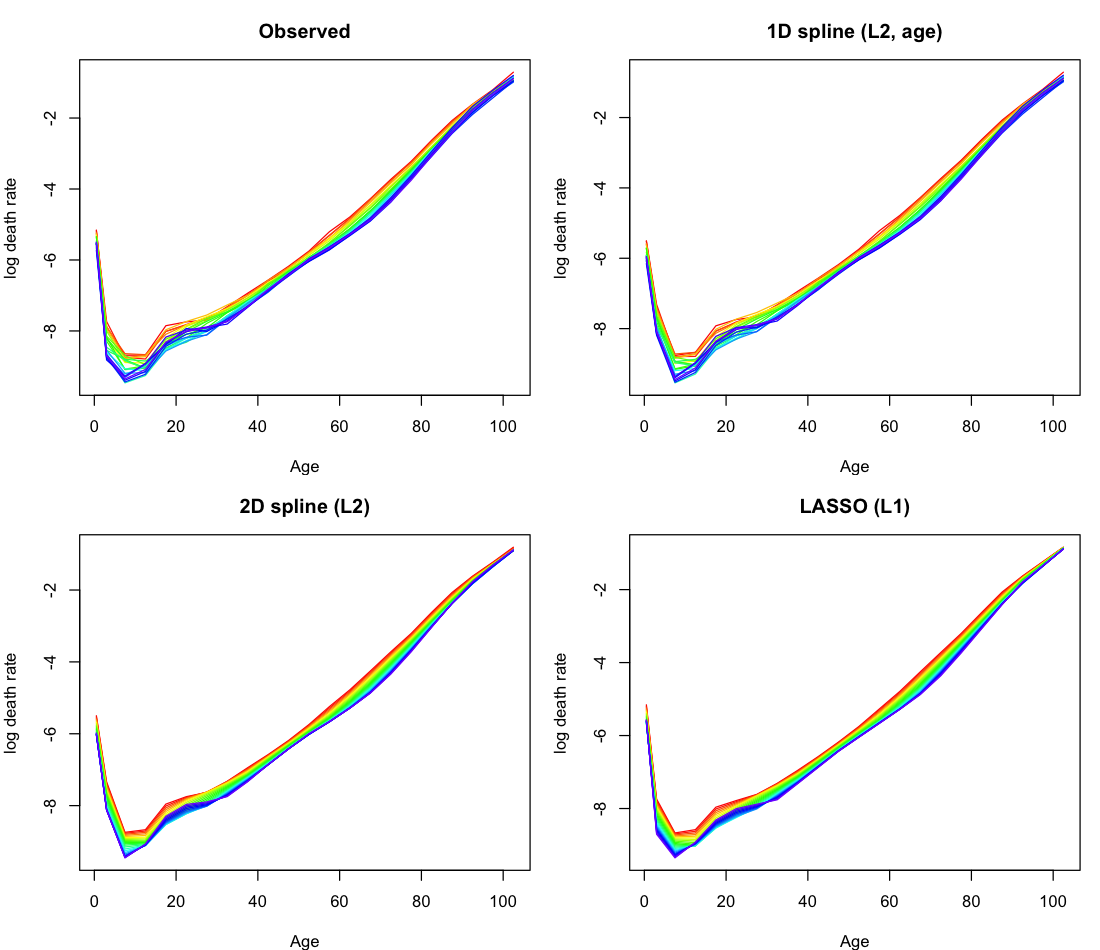
\includegraphics[width=\textwidth]{fig1_smoothing.png}
\end{column}
\end{columns}
\end{frame}

\begin{frame}{\gd{成立 (2)}：$\edag$ 調整使 $\kappa_t$ 更線性}
\begin{columns}[T]
\begin{column}{0.5\textwidth}
\vspace{2pt}
\small
\begin{tabular}{lcc}
\toprule
方法 & drift & 離線性殘差 sd\\
\midrule
LC & $-0.4126$ & 0.9598\\
LCP & $-0.4091$ & 0.7971\\
LM & $-0.4064$ & 0.9071\\
BMS & $-0.4042$ & 0.7864\\
\hi{$\LCe$} & $-0.3593$ & \hi{0.7262}\\
\hi{M$\LCe$} & $-0.3491$ & \hi{0.7026}\\
\bottomrule
\end{tabular}
\vspace{10pt}

\footnotesize
$e_0$ 與 $\edag$ 的反向關係亦成立：\\
$e_0$: $79.64\to83.94$，$\edag$: $11.76\to10.85$，$r=-0.944$。
\end{column}
\begin{column}{0.48\textwidth}
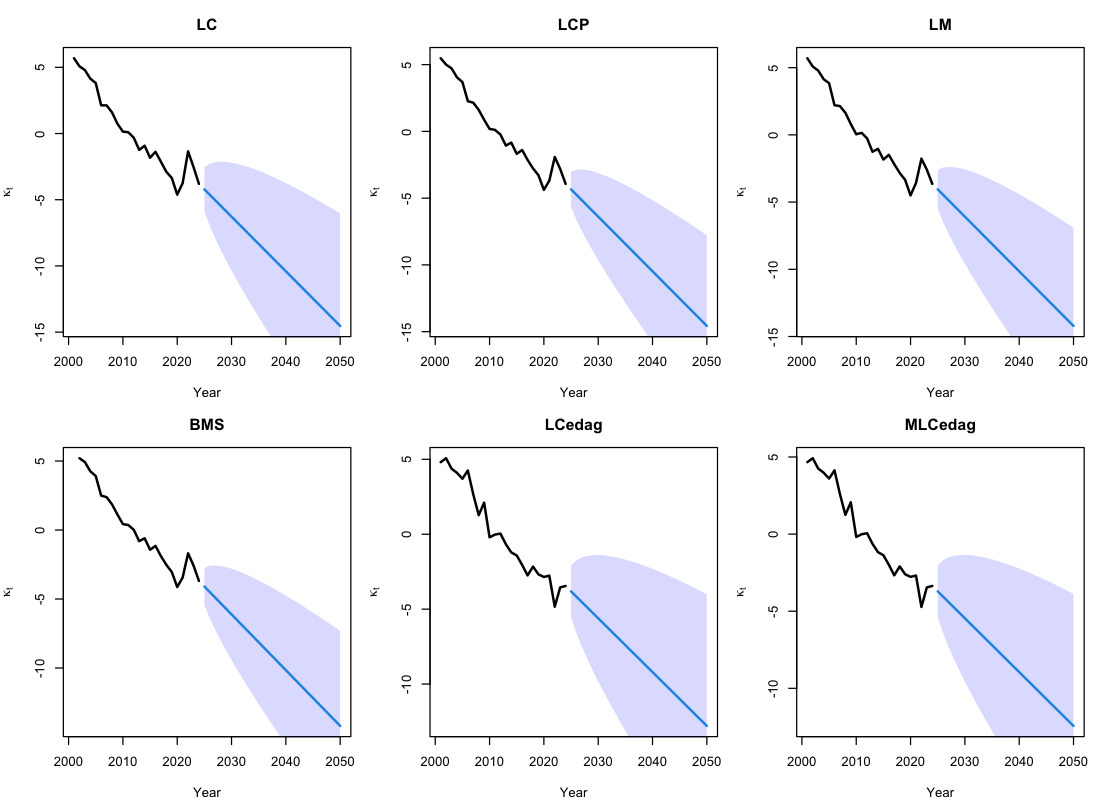
\includegraphics[width=\textwidth]{fig3_kappa.png}
\end{column}
\end{columns}
\end{frame}

\begin{frame}{\gd{成立 (3)}：主分析窗口的樣本外準確度}
女性、2001 起算、留最後 5 年 $\Rightarrow$ $\LCe$ 在\textbf{四個指標上同時最佳}。
\vspace{6pt}
\begin{center}\small
\begin{tabular}{lcccc}
\toprule
方法 & MAE & MSE & MAE($e_0$) & MAE($\edag$)\\
\midrule
LC & 0.1194 & 0.0279 & 0.7969 & 0.1298\\
LCP & 0.1186 & 0.0271 & 0.7976 & 0.1295\\
LM & 0.1080 & 0.0195 & 0.7910 & 0.1035\\
BMS & 0.1172 & 0.0270 & 0.7466 & 0.1293\\
\hi{$\LCe$} & \hi{0.0962} & 0.0160 & \hi{0.6941} & \hi{0.0896}\\
\hi{M$\LCe$} & \hi{0.0962} & \hi{0.0159} & 0.6965 & 0.0897\\
\bottomrule
\end{tabular}
\end{center}
\vspace{8pt}
\begin{alertblock}{但是……}
這是\textbf{一個}窗口的結果。下一頁把它擴充成 12 格面板。
\end{alertblock}
\end{frame}

\section{論文還原：不成立的部分}

\begin{frame}{\hi{不成立 (1)}：優勢僅限於近期短窗口}
擴充成「性別 $\times$ 起始年」12 格面板後，$\LCe$ 的優勢\textbf{並非普遍}：
\vspace{4pt}
\begin{center}\scriptsize
\begin{tabular}{lcccc@{\hspace{10pt}}lcccc}
\toprule
起始年 & $\LCe$ & M$\LCe$ & LM & LC & 起始年 & $\LCe$ & M$\LCe$ & LM & LC\\
\midrule
女 2001 & \gd{0.0962} & \gd{0.0962} & 0.1080 & 0.1194 & 男 1981 & 0.1323 & --- & \hi{0.1099} & 0.1454\\
女 1991 & 0.0992 & \gd{0.0988} & 0.1064 & 0.1197 & 男 1971 & 0.1124 & --- & \hi{0.1078} & 0.1353\\
女 1981 & 0.1194 & 0.1202 & \hi{0.1057} & 0.1163 & 總 2001 & 0.0862 & \gd{0.0841} & 0.0967 & 0.1141\\
女 1971 & 0.1172 & 0.1152 & \hi{0.1061} & 0.1300 & 總 1991 & 0.0945 & \gd{0.0905} & 0.0956 & 0.1266\\
男 2001 & 0.0965 & \gd{0.0942} & 0.1062 & 0.1232 & 總 1981 & 0.1080 & --- & \hi{0.0950} & 0.1268\\
男 1991 & 0.1243 & --- & \hi{0.1090} & 0.1436 & 總 1971 & 0.1005 & --- & \hi{0.0935} & 0.1227\\
\bottomrule
\end{tabular}
\end{center}
\vspace{6pt}
\begin{itemize}\small
  \item $\LCe$/M$\LCe$ 只在 \textbf{5/12 格}勝出（全部是 2001、1991 的短窗口）。
  \item 其餘 \textbf{7/12 格由 LM 奪冠}；1981、1971 的長窗口\textbf{無一例外}。
  \item Total 1970--2024：$\edag$ 調整讓 $\kappa$ \hi{更不線性}（1.824 vs LC 0.848）——方向相反。
\end{itemize}
\vspace{2pt}
\footnotesize\textbf{原文 20 國全部用 1950 年起的長序列，從未檢驗窗口敏感度。}
\end{frame}

\begin{frame}{\hi{不成立 (2)}：預測區間不是更窄而是更寬}
\begin{columns}[T]
\begin{column}{0.52\textwidth}
\vspace{2pt}\small
\begin{tabular}{lcc}
\toprule
方法 & $e_0(2050)$ & 80\% 寬度\\
\midrule
LC & 87.99 & 3.591\\
LCP & 88.02 & \gd{2.875}\\
LM & 87.86 & 3.090\\
BMS & 87.95 & 2.895\\
\hi{$\LCe$} & 87.61 & \hi{3.977}\\
M$\LCe$ & 87.47 & 3.842\\
\bottomrule
\end{tabular}
\vspace{10pt}

\footnotesize
\textbf{原因}：$\kappa$ 更線性 $\ne$ 更低變異。\\[3pt]
$\LCe$ 的一階差 sd $=0.879$，
反而\textbf{略高於} LC 的 $0.851$。\\[3pt]
\hi{原文把這兩件事綁在一起論述。}
\end{column}
\begin{column}{0.46\textwidth}
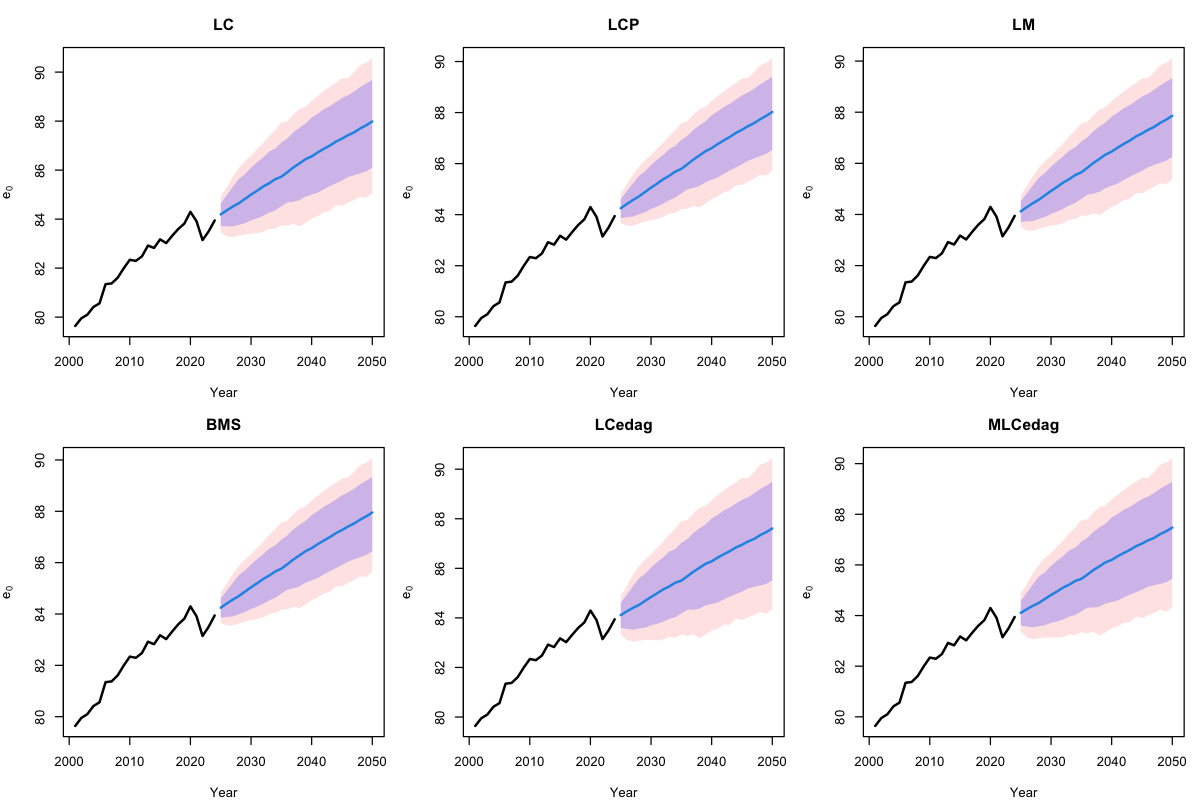
\includegraphics[width=\textwidth]{fig9_e0_forecast.png}
\end{column}
\end{columns}
\end{frame}

\begin{frame}{\hi{不成立 (3)}：涵蓋率的優勢是買來的}
\begin{itemize}
  \item $\LCe$ 的涵蓋機率偏差最低（0.20），但平均區間寬度 \textbf{1.391}
        是 LC 的 \textbf{0.875} 的 \hi{1.6 倍}。
  \item 更重要的是：\hi{六種方法的實證涵蓋率都在 0.2--0.6，離名目 0.8 都很遠。}
\end{itemize}
\vspace{6pt}
\begin{center}
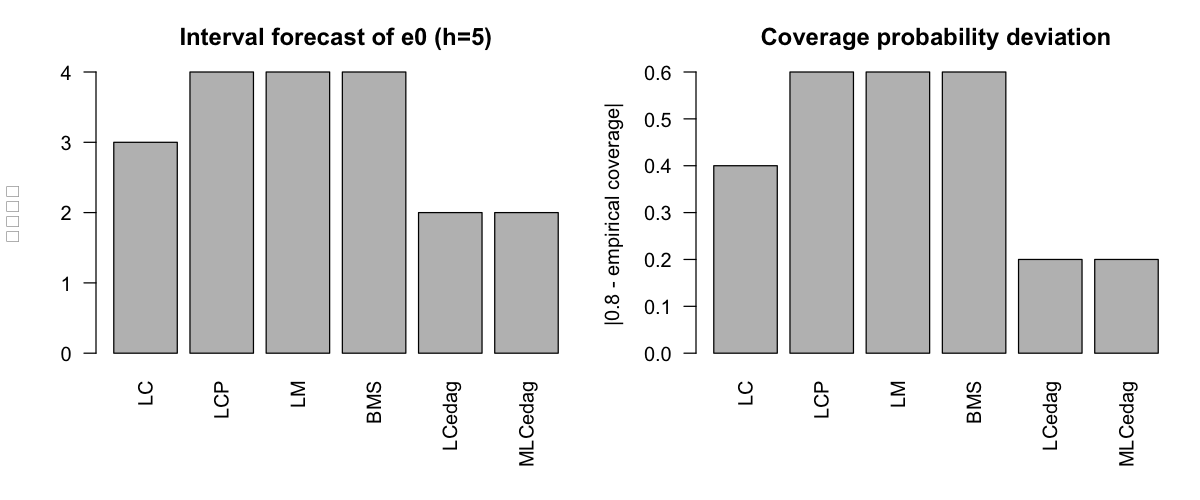
\includegraphics[width=0.72\textwidth]{fig10_coverage.png}
\end{center}
\vspace{2pt}
\footnotesize
方向與 Shang 等人 (2011)「十種擴充全部低估變異性」一致，
但本研究是在\textbf{單一人口、五齡組、含 COVID 的留出期}上得到的，程度嚴重得多。
\end{frame}

\begin{frame}{論文還原過程浮現的三個方法論問題}
\begin{block}{(1) 原文 Fig.~8 的相關係數是\hi{受模型結構決定}}
\small 秩 1 的 LC 中每年整條曲線由單一純量 $\kappa_t$ 決定
$\Rightarrow$ $e_0$ 與 $\edag$ 必然都是 $\kappa_t$ 的單調函數、近乎完美相關
（配適值 $r=-0.999$）。\textbf{據此比較 $r$ 值的論證站不住腳。}
\end{block}
\begin{block}{(2) $\edag$ 對 $\kappa$ 是\hi{單峰而非單調}}
\small $\edag(\kappa)$ 在 $\kappa\approx54$ 有峰值 30.2，兩側遞減
$\Rightarrow$「以 $\edag$ 對齊 $\kappa$」\textbf{原則上可能有兩個解}。
低死亡率國家碰不到，但高死亡率人口或極端外推未必。\textbf{原文完全未討論。}
\end{block}
\begin{block}{(3) 原文選修勻參數的準則\hi{在台灣數據上傾向選擇「不修勻」}}
\small 以對觀測值的 MAE/MSE 為準則，而修勻\textbf{依定義}必然增加對觀測值的誤差。
$\Rightarrow$ 這不是方法比較，是準則的定義決定的。
\end{block}
\end{frame}

\section{延伸研究}

\begin{frame}{延伸 (1)：暴露數的蒙地卡羅實驗}
以女性 2001--2024 的配適為真值，$D_{x,t}\sim\text{Poisson}(E_{x,t}m^{\text{true}}_{x,t})$，
$E=N\cdot w$。
\vspace{4pt}
\begin{center}\small
\begin{tabular}{rcccc}
\toprule
$N$ & 零格/528 & $\alpha$ 偏誤 & $\beta$ 相關（LC / LASSO） & drift 中位數\\
\midrule
10,000 & 214.6 & \hi{$+0.441$} & $-0.275$ / $-0.435$ & $-0.110$\\
50,000 & 88.9 & $+0.033$ & $-0.128$ / $-0.030$ & $-0.078$\\
200,000 & 21.8 & $-0.051$ & $+0.553$ / $+0.574$ & $-0.287$\\
1,000,000 & 0.4 & $-0.017$ & $+0.830$ / $+0.865$ & $-0.315$\\
\bottomrule
\end{tabular}
\end{center}
\vspace{4pt}
\footnotesize（drift 真值 $-0.3678$；管線本身無誤：$N=10^8$ 時相關 0.999。）
\vspace{4pt}
\begin{itemize}\footnotesize
  \item $N\le2\times10^4$：零格佔四成，\hi{主導一切的是零格處理而非估計方法}。
  \item $N\le2\times10^5$：兩種方法的 $\beta$ \hi{都已崩潰}。
  \item \hi{drift 被系統性壓平}——有方向的偏誤，直接乘上預測期長度進入 $e_0$。
  \item LASSO 最明確的貢獻是\gd{把 drift 拉回真值附近並使四分位距減半}。
\end{itemize}
\end{frame}

\begin{frame}{延伸 (1)：圖示}
\begin{center}

\includegraphics[height=0.80\textheight]{mc_plots.png}
\end{center}
\end{frame}

\begin{frame}{延伸 (2)：$\lambda$ 的選擇與三個方向}
\begin{columns}[T]
\begin{column}{0.47\textwidth}
\textbf{交叉驗證在最需要它的地方失效}
\begin{itemize}\small
  \item 大人口命中，小人口\hi{修勻不足七倍}。
  \item 原因：CV 衡量\textbf{曲面}的預測誤差，
        而 $\beta$ 是曲面的\textbf{泛函}、對雜訊敏感得多。
  \item $\lambda=0$ \hi{根本無法被交叉驗證}
        $\Rightarrow$ 回答不了「要不要修勻」。
  \item 改用\gd{參數式 bootstrap 插入式選法}明顯較好。
\end{itemize}
\end{column}
\begin{column}{0.5\textwidth}
\textbf{三個方向拆開}（$N=2\times10^5$）
\vspace{2pt}
\begin{center}\scriptsize
\begin{tabular}{cccrr}
\toprule
$\lambda_{xx}$ & $\lambda_{xt}$ & $\lambda_{tt}$ & SSE($\beta$) & SSE($\alpha$)\\
\midrule
20 & 2 & 1 & 0.0065 & 5.131\\
1 & 2 & 20 & 0.0069 & 0.219\\
\gd{1} & \gd{2} & \gd{1} & \gd{0.0075} & \gd{0.203}\\
0 & 0 & 0 & 0.0483 & 0.296\\
20 & 0 & 0 & \hi{0.1235} & 5.976\\
\bottomrule
\end{tabular}
\end{center}
\vspace{4pt}
\footnotesize
\hi{$\lambda_{xt}$ 是主力}：在 LC 底下
$\partial^2\log m/\partial x\partial t=\beta'_x\kappa'_t$，
交叉項\textbf{本質上就是對 $\beta_x$ 粗糙度的懲罰}，
是三個方向裡唯一直接瞄準 $\beta$ 的。
\end{column}
\end{columns}
\end{frame}

\begin{frame}{延伸 (3)：區間的不確定性來源分解\quad\small（$h=10$，名目 80\%）}
\begin{center}\small
\begin{tabular}{rlcc}
\toprule
$N$ & 變體 & 平均寬度 & 涵蓋率\\
\midrule
50,000 & O\ 只有未來創新（\textbf{不可約下限}） & 1.743 & 0.85\\
 & P\ 插入式（\textbf{現行做法}） & \hi{5.401} & \hi{0.38}\\
 & S\ 修勻＋參數不確定性 & 1.683 & 0.66\\
\midrule
1,000,000 & O & 1.738 & 0.77\\
 & P & 4.390 & 0.94\\
 & S & 1.194 & \hi{0.45}\\
\midrule
11,900,000 & O & 1.723 & 0.87\\
 & S & \hi{0.529} & \hi{0.38}\\
\bottomrule
\end{tabular}
\end{center}
\vspace{4pt}
\begin{itemize}\footnotesize
  \item \hi{小人口的區間同時「太寬」且「涵蓋不足」}——寬度與涵蓋\textbf{解耦}。
        \textbf{問題是偏誤，不是寬度；加寬區間無濟於事。}
  \item bootstrap 的參數不確定性\hi{幾乎無貢獻}：它繞著\textbf{已經偏掉}的配適值重抽，
        偵測不到自己的偏誤。
  \item \hi{修勻讓區間系統性過窄，且 $N$ 越大越嚴重}（$0.66\to0.45\to0.38$）。
\end{itemize}
\end{frame}

\begin{frame}{延伸 (4)：兩步校正}
\begin{block}{步驟一（位置）：以卜瓦松 MLE 取代 SVD}
\small
\begin{center}
\begin{tabular}{rcc}
\toprule
$N$ & SVD 的 drift & 卜瓦松 MLE 的 drift\\
\midrule
50,000 & $-0.032$（偏誤 \hi{$+0.336$}） & \gd{$-0.377$}（偏誤 $-0.010$）\\
200,000 & $-0.194$（偏誤 \hi{$+0.174$}） & \gd{$-0.369$}（偏誤 $-0.002$）\\
\bottomrule
\end{tabular}
\end{center}
\vspace{2pt}
\hi{drift 衰減不是小人口的固有性質，而是 SVD 對 $\log(D/E)$ 做最小平方的產物。}
卜瓦松不取對數，衰減消失。
\end{block}
\begin{block}{步驟二（寬度）：以 bootstrap 去除 $\hat\sigma$ 中的估計雜訊}
\small
$\widehat{\text{Var}}(\Delta\hat\kappa)\approx\sigma^2+\text{Var}(\Delta u)$，
扣除後（真值 $\sigma=0.7496$）：
$N=2\times10^5$ 時 $1.152\to\gd{0.702}$；$N=10^6$ 時 $0.870\to\gd{0.751}$。\\
\footnotesize 操作邊界：$N=5\times10^4$ 時 $\sqrt{V_u}=7.36>\hat\sigma_{\text{naive}}=2.30$，
兩個大噪音相減不穩定 $\Rightarrow$ 去偏約在 $N\ge2\times10^5$ 可行。
\end{block}
\end{frame}

\begin{frame}{兩步合併後的校準結果}
\begin{center}\small
\begin{tabular}{rlcc}
\toprule
$N$ & & 寬度 & 涵蓋率（名目 0.80）\\
\midrule
200,000 & oracle & 1.743 & 0.81\\
 & 現行做法 & 5.081 & 0.75\\
 & \gd{校準版} & \gd{1.724} & 0.63\\
\midrule
1,000,000 & oracle & 1.726 & 0.85\\
 & 現行做法 & 4.667 & 0.95\\
 & \gd{校準版} & \gd{1.721} & \gd{0.83}\\
\midrule
11,900,000 & oracle & 1.712 & 0.78\\
 & 現行做法 & 2.033 & 0.82\\
 & \gd{校準版} & \gd{1.678} & 0.77\\
\bottomrule
\end{tabular}
\end{center}
\vspace{8pt}
\begin{itemize}\small
  \item $N\ge10^6$ 時\gd{校準版寬度幾乎完全追上不可約下限}，涵蓋率 0.83 對名目 0.80。
  \item 現行做法在同一點的「涵蓋 0.95」是靠 \hi{2.7 倍寬度}換來的，\textbf{不是校準良好}。
  \item \textbf{尚未解決}：$N=2\times10^5$ 時寬度已對但涵蓋僅 0.63，
        殘餘位置誤差來自 $\hat\kappa_T$ 這個\textbf{起點}本身。
\end{itemize}
\end{frame}

\section{懲罰式 Lee-Carter}

\begin{frame}{懲罰式 LC：收縮目標必須是非零向量}
\begin{alertblock}{實作上的關鍵前提}
\small
在 LC 的識別條件 $\sum_x\beta_x=1$ 之下，
\[
\sum_x|\beta_x|=\sum_x\beta_x+2\sum_x\max(-\beta_x,0)=1+2\sum_x\max(-\beta_x,0)
\]
$L_1$ 懲罰\hi{只罰 $\beta_x$ 的負部}。當 $\hat\beta_x$ 全為正（大人口必然如此），
$\sum|\beta_x|\equiv1$ 是常數 $\Rightarrow$ \hi{估計值完全不動。}
\end{alertblock}
\vspace{2pt}
\begin{center}\scriptsize
\begin{tabular}{rcccc}
\toprule
& \multicolumn{2}{c}{$\beta_0=\mathbf{0}$} & \multicolumn{2}{c}{$\beta_0=\mathbf{1}/A$}\\
\cmidrule(lr){2-3}\cmidrule(lr){4-5}
$\lambda$ & $\max|\hat\beta-\hat\beta^{\text{unpen}}|$ & 自由參數
          & $\max|\hat\beta-\hat\beta^{\text{unpen}}|$ & 自由參數\\
\midrule
$10^2$ & \hi{$9.0\times10^{-17}$} & 22 & 0.0041 & 19\\
$10^4$ & \hi{$1.5\times10^{-16}$} & 22 & 0.0612 & \gd{6}\\
$10^6$ & \hi{$2.1\times10^{-15}$} & 22 & 0.0612 & \gd{0}\\
\bottomrule
\end{tabular}
\end{center}
\vspace{3pt}
\footnotesize
$\Rightarrow$ 本文取 $\beta_0=\mathbf{1}/A$：滿足 $\sum\beta_0=1$ 故懲罰非退化，
意義為\gd{「各年齡等速改善」的虛無假設}，
LASSO 的稀疏性即回答\gd{「哪些年齡顯著偏離平均」}。
\end{frame}

\begin{frame}{演算法與收斂}
\begin{columns}[T]
\begin{column}{0.44\textwidth}
\small
區塊座標下降：$\alpha$ 封閉解、$\kappa$ Newton、
$\beta$ 用 proximal Newton
\[
\beta_x=\beta_{0x}+\frac{S(W_x(\tilde\beta_x-\beta_{0x})-\nu,\ \lambda a w_x)}
{W_x+\lambda(1-a)w_x}
\]
\footnotesize
不可微項只在 $\beta$ 一個區塊、且各年齡可分離
$\Rightarrow$ \textbf{Tseng (2001)} 的收斂定理適用。
\vspace{6pt}

\begin{tabular}{rcc}
\toprule
$\lambda$ & 迭代次數 & 收斂\\
\midrule
$0$ & 33 & 是\\
$10^3$ & 18 & 是\\
$10^4$ & \gd{6} & 是\\
\bottomrule
\end{tabular}
\vspace{4pt}

\gd{懲罰越強收斂越快}（改善條件數）。
\end{column}
\begin{column}{0.54\textwidth}
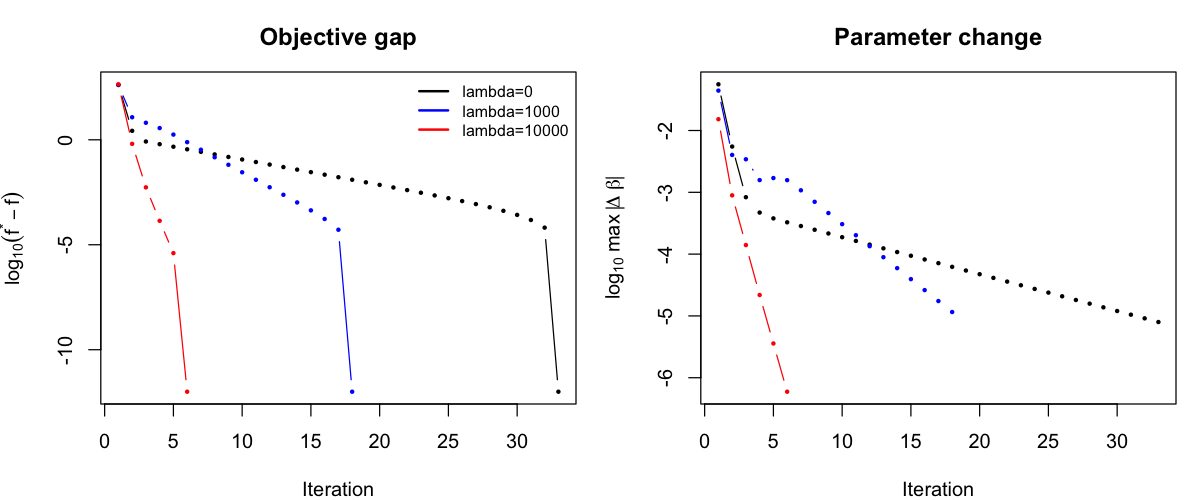
\includegraphics[width=\textwidth]{fig1_convergence.png}
\\[2pt]
\footnotesize 兩者皆線性下降 $\Rightarrow$ \textbf{幾何收斂}。
\end{column}
\end{columns}
\end{frame}

\begin{frame}{係數路徑：$\lambda$ 增大時 $\beta_x$ 依序併入 $1/A$}
\begin{center}
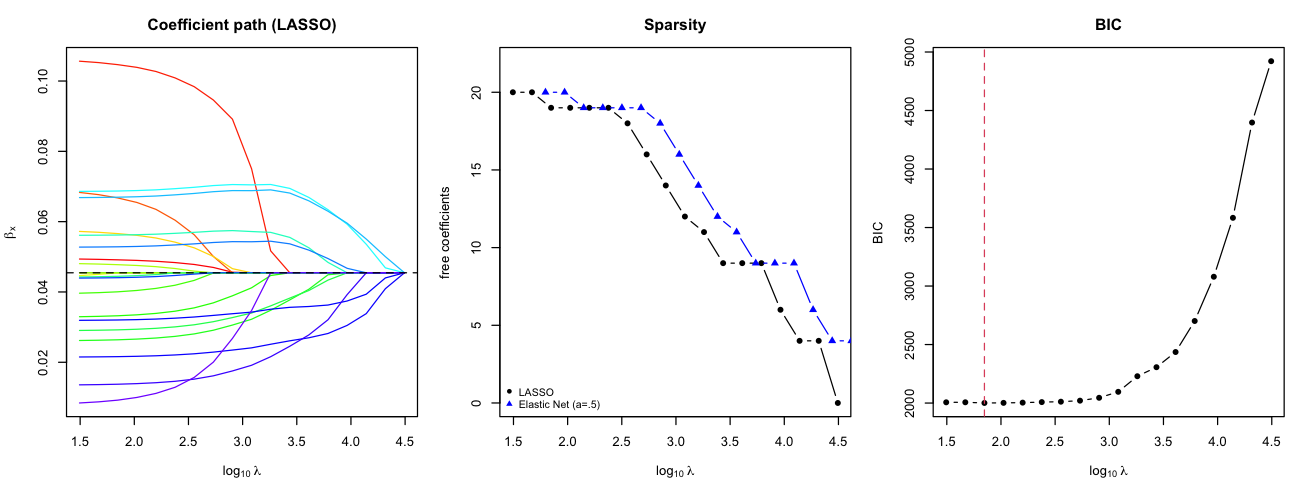
\includegraphics[width=\textwidth]{fig2_path.png}
\end{center}
\vspace{-2pt}
\begin{itemize}\footnotesize
  \item 中圖：Elastic Net 稀疏化較慢 = \textbf{Zou \& Hastie (2005) 的群組效應}
        （相鄰年齡的 $\beta_x$ 高度相關，$L_2$ 項使整組一同保留）。
  \item 右圖：BIC 在全國女性（約 1,190 萬人）偏好小 $\lambda$ ——
        \hi{懲罰的價值須在小人口才顯現}。
\end{itemize}
\end{frame}

\begin{frame}{偏誤—變異數權衡}
\begin{columns}[T]
\begin{column}{0.54\textwidth}
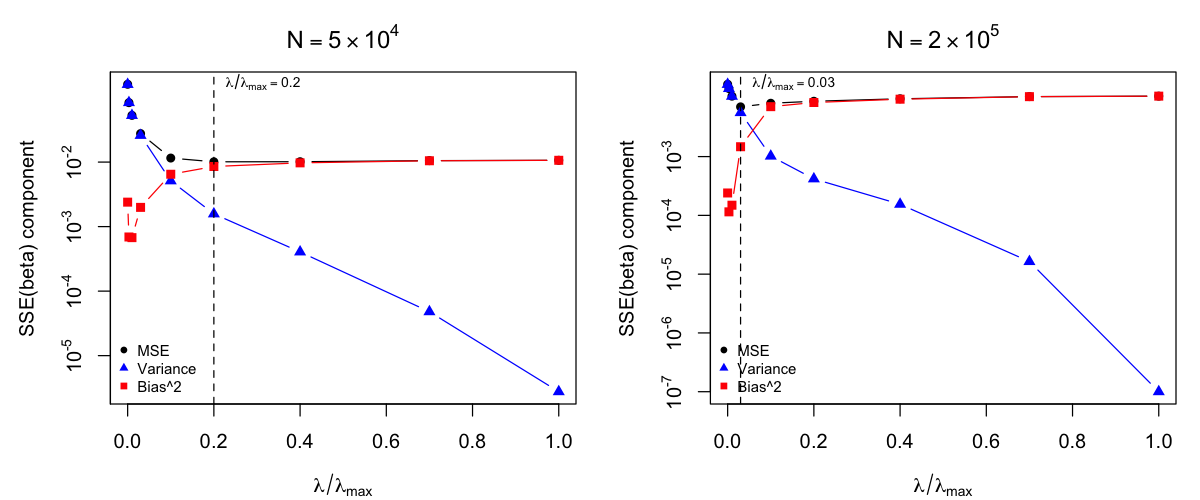
\includegraphics[width=\textwidth]{fig3_bias_variance.png}
\end{column}
\begin{column}{0.44\textwidth}
\vspace{4pt}\scriptsize
\begin{tabular}{rcccc}
\toprule
$N$ & $\lambda/\lambda_{\max}$ & 偏誤$^2$ & 變異數 & MSE\\
\midrule
5 萬 & 0 & .0024 & .1598 & .1606\\
     & \gd{0.20} & .0085 & .0016 & \gd{.0101}\\
\midrule
20 萬 & 0 & .0002 & .0169 & .0170\\
      & \gd{0.03} & .0015 & .0056 & \gd{.0070}\\
\bottomrule
\end{tabular}
\vspace{8pt}

\footnotesize
$N=5$ 萬：MSE \gd{降 94\%}、變異數降 99\%。\\[4pt]
即 \textbf{James \& Stein (1961)}「以偏誤換變異數」的古典結果。\\[4pt]
\hi{最適 $\lambda$ 隨 $N$ 增大而下降}（0.20 $\to$ 0.03）。
\end{column}
\end{columns}
\vspace{2pt}
\footnotesize
\textbf{註}：$\lambda$ 須以 $\lambda_{\max}$ 正規化——Hessian 尺度正比於 $N$，
絕對尺度的 $\lambda$ 跨暴露數不可比。
\end{frame}

\begin{frame}{變異數的收斂速度與 MSE 的交叉}
\begin{center}
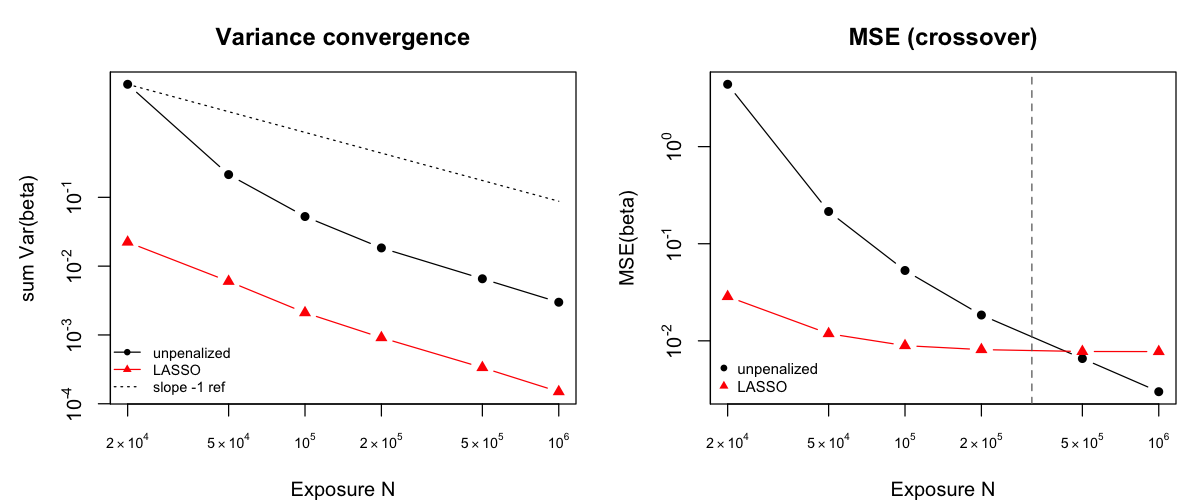
\includegraphics[width=0.78\textwidth]{fig4_variance_rate.png}
\end{center}
\vspace{-2pt}
\begin{itemize}\footnotesize
  \item \textbf{懲罰縮小的是變異數的「常數項」，不是收斂階數}：
        $N=2$ 萬時 4.391 vs 0.022（\gd{差 197 倍}），
        但 log-log 斜率 $-1.77$ vs $-1.27$，無階數差異。
  \item 未懲罰版斜率的標準誤 0.22（懲罰版 0.04）$\Rightarrow$ 小 $N$ 並非穩定冪次，
        而是處於\hi{崩潰區}，「斜率較陡」是脫離崩潰的過渡，不是收斂較快。
  \item \hi{固定比例的懲罰在 $N\ge3\times10^5$ 後反而有害}（偏誤不隨 $N$ 消失）
        $\Rightarrow$ $\lambda$ 必須隨人口規模調整。
\end{itemize}
\end{frame}

\begin{frame}{LASSO vs Ridge vs Elastic Net（$N=20$ 萬）}
\begin{center}\small
\begin{tabular}{lccccc}
\toprule
懲罰 & 最適 $\lambda/\lambda_{\max}$ & 偏誤$^2$ & 變異數 & MSE & $\beta$ 相關\\
\midrule
未懲罰 & 0 & .00024 & .01691 & .01698 & .711\\
LASSO & 0.030 & .00147 & .00560 & .00702 & .703\\
Elastic Net & 0.030 & .00158 & .00534 & .00687 & .705\\
Ridge & 0.003 & .00270 & .00311 & \gd{.00578} & \gd{.721}\\
\bottomrule
\end{tabular}
\end{center}
\vspace{6pt}
\begin{itemize}\small
  \item MSE 分別降低 59\%、60\%、\gd{66\%}。
  \item \hi{若純看 MSE，Ridge 最佳、LASSO 最差}——真值 $\beta_x$ 沒有任何一組
        恰等於 $1/A$，\textbf{稀疏性並非正確的先驗}。
  \item 但 LASSO 提供 Ridge 沒有的\gd{變數選擇與可解釋性}
        （$\lambda=10^4$ 時僅 6 組維持自由）。
        \textbf{以約 20\% 的 MSE 換取可解釋性，取捨視研究目的而定。}
  \item 目的為\textbf{估計精確度} $\Rightarrow$ Ridge／Elastic Net；
        目的為\textbf{辨識關鍵年齡} $\Rightarrow$ LASSO。
\end{itemize}
\end{frame}

\begin{frame}{配適期長度 $T$ 比人口規模 $N$ 更關鍵}
以女性 1970--2024（55 年）為真值，$T\times N$ 二因子，各 100 次。
\textbf{指標用 cor$(\hat\beta,\beta^{\text{true}})$ 而非 SSE}——
$T$、$N$ 都小時 $\hat\beta$ 會\hi{完全塌陷為 $\mathbf{1}/A$}，
此時 SSE 反而「看起來很好」。
\vspace{3pt}
\begin{columns}[T]
\begin{column}{0.46\textwidth}
\centering\scriptsize
cor$(\hat\beta,\beta^{\text{true}})$ 中位數\\[2pt]
\begin{tabular}{rcccc}
\toprule
$T$ & $2\!\times\!10^4$ & $5\!\times\!10^4$ & $2\!\times\!10^5$ & $10^6$\\
\midrule
10 & 0.25 & 0.16 & 0.17 & \hi{0.12}\\
20 & 0.18 & 0.22 & 0.41 & 0.76\\
30 & 0.32 & 0.59 & 0.79 & \gd{0.95}\\
40 & 0.51 & 0.73 & \gd{0.90} & \gd{0.98}\\
55 & \gd{0.75} & \gd{0.87} & \gd{0.97} & \gd{0.99}\\
\bottomrule
\end{tabular}
\vspace{5pt}

\scriptsize 退化率（塌陷為 $\mathbf{1}/A$）：
$T{=}10,N{=}2\!\times\!10^4$ 時達 \hi{81\%}。
\end{column}
\begin{column}{0.52\textwidth}
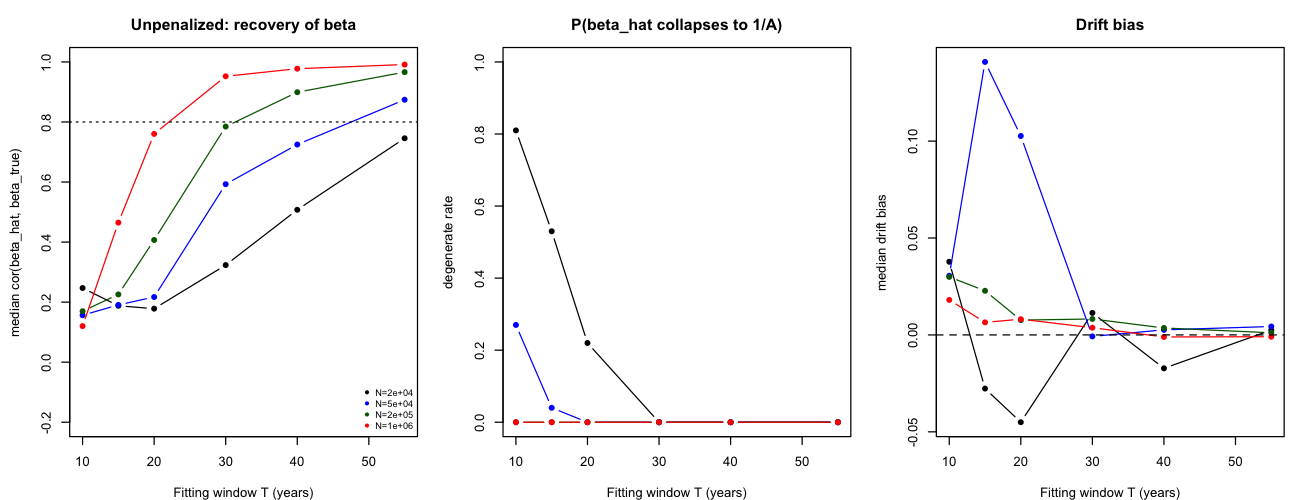
\includegraphics[width=\textwidth]{figB_TxN.png}
\end{column}
\end{columns}
\vspace{3pt}
\begin{itemize}\footnotesize
  \item \hi{$T=10$ 年時即使 $N=10^6$ 也只有 0.12}；$T=55$ 年時 $N$ 僅 2 萬也有 0.75。
        \gd{「長窗口配小人口」勝過「短窗口配大人口」}。
  \item 以 0.8 為門檻：$T{=}55$ 需 $N\!\ge\!5$ 萬、$T{=}40$ 需 20 萬、$T{=}30$ 需 100 萬；
        \hi{$T\le20$ 年時任何人口規模都達不到}。
\end{itemize}
\end{frame}

\begin{frame}{Elastic Net 族的其他變體}
針對「LASSO 的弱點是偏誤」，另試三種以降低收縮偏誤為目的的變體：
\vspace{3pt}
\begin{center}\small
\begin{tabular}{lcccc}
\toprule
方法 & 最適 $\lambda/\lambda_{\max}$ & 偏誤$^2$ & 變異數 & MSE\\
\midrule
Ridge & 0.003 & .00270 & .00311 & \gd{.00578}\\
LASSO & 0.03 & .00219 & .00484 & .00698\\
MCP ($\gamma=3$) & 0.03 & .00219 & .00485 & .00698\\
Elastic Net & 0.10 & .00463 & .00255 & .00716\\
自適應 LASSO & 0.40 & .00313 & .00532 & .00840\\
鬆弛 LASSO & 0.20 & .00734 & \gd{.00192} & \hi{.00924}\\
\bottomrule
\end{tabular}
\end{center}
\vspace{4pt}
\begin{itemize}\footnotesize
  \item \hi{沒有任何稀疏型變體勝過單純的 Ridge}——真值是\textbf{稠密}的，
        為稀疏性設計的機制無從發揮。
  \item \textbf{MCP $\approx$ LASSO}：最適 $\lambda$ 下閾值本就小，
        MCP「對大係數不加偏誤」的區段極少觸發。
  \item \textbf{鬆弛 LASSO 變異數最低卻 MSE 最差}：把非作用集\textbf{硬性固定}
        於 $\beta_0$ 是過強的等式限制。
\end{itemize}
\end{frame}

\section{定位與下一步}

\begin{frame}{四項議題}
\begin{enumerate}\small\setlength{\itemsep}{7pt}
  \item \textbf{小樣本研究多針對變異數，對 SVD 的偏誤著墨較少。}
        Chen et al.\ (2017) 已系統探討人口規模對 MLE 有限樣本分布的影響，
        但對象是 M7 模型、估計自始為\textbf{卜瓦松 MLE}，聚焦
        \textbf{參數不確定性}；而本文顯示 MLE 的漂移項幾乎無偏誤，
        \hi{真正有系統性偏誤的是 LC 預設的 SVD}——既有設計看不到此現象。
  \item \textbf{修勻壓低區間寬度已被指出，卻無人量化。}
        該回顧討論節明確提出並\textbf{點名五齡組}，但未提供任何量化證據。
  \item \textbf{平滑參數的選擇準則與估計目標錯置。}
        Delwarde et al.\ (2007) 用交叉驗證、Rabbi and Mazzuco 用對觀測值的誤差；
        前者小人口修勻不足七倍、後者在台灣數據上傾向選擇不修勻。
  \item \hi{\textbf{時間參數 $\kappa_t$ 在小人口的行為尚未被檢驗。}}
        此點由 \textbf{Yue et al.\ (2019)} 於結論中明白指出。
        然而 $\kappa_t$ 的漂移項\textbf{直接乘上預測期長度}進入平均餘命，
        其偏誤對長期預測的影響遠大於年齡參數。
\end{enumerate}
\vspace{4pt}
\centerline{\small 本文針對\textbf{議題二至議題四}提出量化證據。}
\end{frame}

\begin{frame}{必須主動說明的限制}
\begin{enumerate}\small\setlength{\itemsep}{6pt}
  \item \textbf{五齡組本身是強力的變異數縮減器}（最小格死亡數 37、中位數 1201）。
        得到的是「五齡組之下」的門檻，不能與單齡組研究直接比較。
  \item \textbf{時間窗長度與人口規模是兩個獨立、且會相乘的脆弱來源。}
        24 年窗口的 $\kappa$ 總變化僅 8.8 個單位，55 年則有 22 個。
  \item \textbf{蒙地卡羅的真值取自 LC 配適}，隱含「模型正確」假設；
        真實小人口的 $\beta_x$ 可能本就不同於全國 $\Rightarrow$ 模擬給的是\textbf{下界}。
  \item \textbf{涵蓋率的實證驗證本身有困難}（Alho \& Spencer 2005）。
  \item \textbf{留出期含 COVID}（女性 $e_0$: 2020 年 84.30 $\to$ 2022 年 83.14
        $\to$ 2024 年 83.94），屬真實結構性衝擊。
  \item \textbf{部分模擬的重複次數尚未統一}（reps 10--120），正式版將統一重跑。
\end{enumerate}
\end{frame}

\begin{frame}{下一步工作}
\begin{enumerate}\setlength{\itemsep}{8pt}
  \item \textbf{統一模擬規模}：所有蒙地卡羅以 reps $\ge100$ 重跑、固定種子。
  \item \textbf{把 $T$ 納入設計}：改為 $T\times N$ 二因子，分離時間窗長度與人口規模。
  \item \textbf{COVID 對照組}：補跑 2001--2019 並列。
  \item \textbf{單齡組檢驗}：分離「五齡組近似誤差」與「台灣死亡轉型較快」
        這兩個競爭解釋。
  \item \textbf{jump-off 的取捨}：量化 Stoeldraijer 等人 (2018) 的準確度／穩健度
        取捨在小人口下的位置——這是目前殘餘涵蓋誤差的主要來源。
\end{enumerate}
\end{frame}

\begin{frame}{請老師指教}
\vspace{4pt}
\begin{block}{想請教的三個方向}
\begin{enumerate}\setlength{\itemsep}{8pt}
  \item 論文主軸要放在\textbf{議題二}（修勻壓低區間寬度）
        還是\textbf{議題四}（$\kappa_t$ 的偏誤而非變異）？
  \item 懲罰式 LC 的收縮目標，下一步是否由均勻向量 $\mathbf{1}/A$ 改為
        \textbf{實際參考母體的 $\hat\beta^{\text{ref}}$}，以銜接
        \textbf{Yue et al.\ (2019)} 建議的「依年齡選擇參考母體」？
  \item 既然純看 MSE 時 Ridge 優於 LASSO，論文要以\textbf{估計精確度}
        還是\textbf{年齡組的可解釋性}為主要訴求？
  \item 是否值得把\textbf{單齡組}資料納入，以分離五齡組的近似誤差？
\end{enumerate}
\end{block}
\vspace{6pt}
\begin{center}
\footnotesize 程式碼與可重現的圖表：\texttt{github.com/rickyllin/-20260908}
\end{center}
\end{frame}

\end{document}
